\documentclass[12pt]{amsart}
\usepackage[margin=1in]{geometry}
%\usepackage{tikz}
%\usetikzlibrary{calc}
\usepackage{amsmath, amsthm, amssymb, graphicx, setspace}
\usepackage{mymacros}
\usepackage{pysyntax}
\usepackage{verbatim}
\usepackage{hyperref}
\usepackage{graphicx}
\usepackage{caption}
\usepackage{subcaption}
\usepackage{multicol}

\newcommand{\kry}{\mathcal K}
\newcommand{\figref}[1]{\figurename~\ref{#1}}
\DeclareMathOperator*{\argmin}{arg\,min}
\newenvironment{Figure}{\par\medskip\noindent\minipage{\linewidth}}{\endminipage\par\medskip}
\renewcommand{\hat}{\widehat}

\title{Parametric entropy based density estimation in distance sampling}
\author{Kevin Joyce}
\date{12 December 2014} 

\begin{document}
\maketitle
\begin{multicols}{2}
\section{Introduction}
  
  The problem of interest in this work is to estimate the density of objects from distance data collected along line-transects within a given area.
This problem has been extensively studied, and much work involves estimation based on the density estimator
  \begin{equation}
    \hat D_i = \frac {y_i \hat f(0)}{2L_i}
  \end{equation}
  where $y_i$ are the total observation counts for the $i$th transect, $L_i$ is the length of the $i$th transect, and $\hat f$ is an estimated density function modeling detectability based on perpendicular distance from the transect.
In particular, $f$ is such that the proportion of objects observed within a distance of $x$ of any given transect is $\int_0^x f(t)\,dt$.
The density estimator can be derived solely from data that records an observation's perpendicular distance from the transect.
For a derivation see \cite{buckland2001introduction} \cite{thompson2012sampling}.
By far, the most involved part of the estimation is obtaining $\hat f(0)$.

In \cite{buckland2001introduction}, Buckland highlights this difficulty with distance data obtained by Anderson and Pospahala measuring distances of duck nests from a single transect in the Monte Vista National Wildlife Refuge in Colorado.
\begin{Figure}
  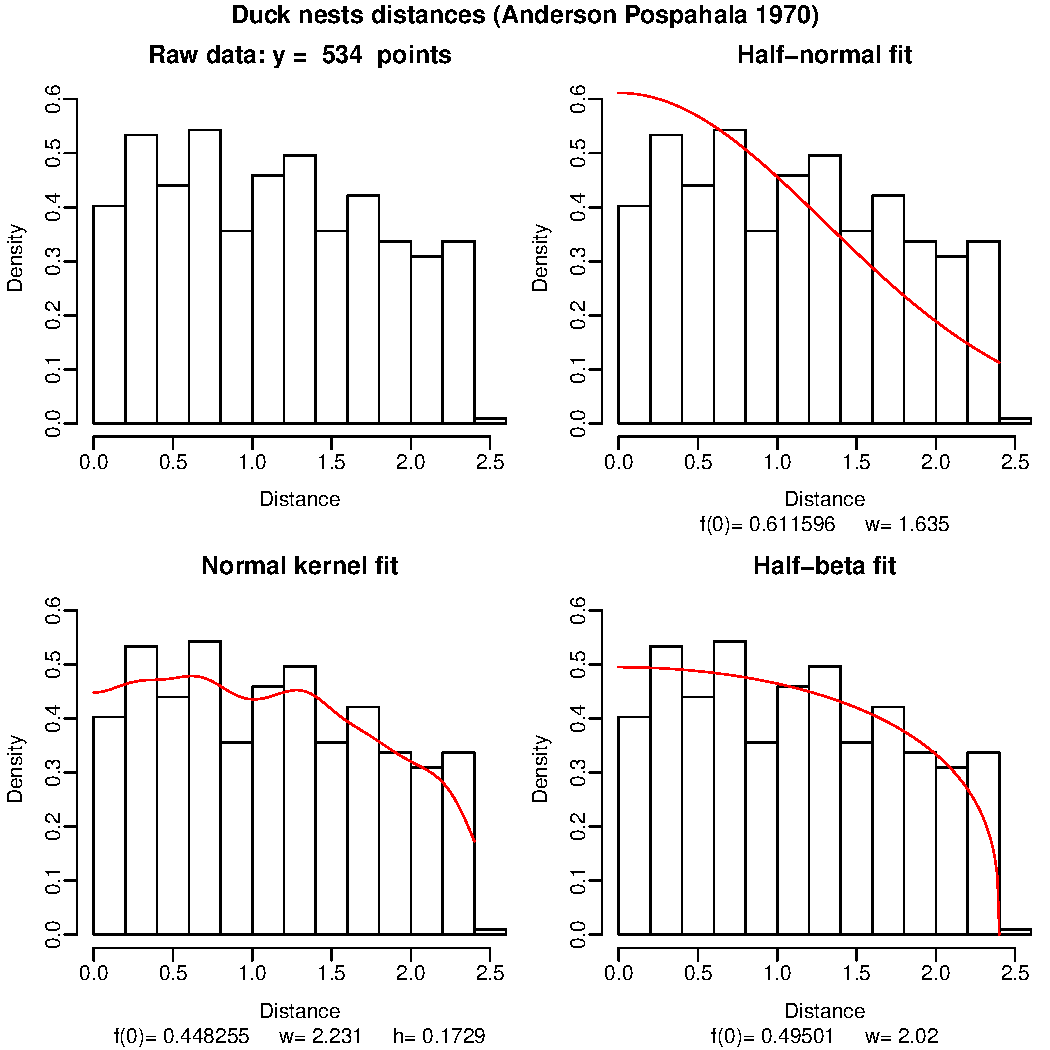
\includegraphics[width=\linewidth]{../duck_nest_fits.pdf}
    \label{duckfits}
    \captionof{figure}{Distance data for duck nests in the Monte Vista National Wildlife Refuge in Colorado.}
\end{Figure}
In \figref{duckfits}, a histogram of the distance data is displayed with a parametric half-normal density fit, a non-parametric normal kernel fit, and a density fit using the method described in this work.
Note that the abrupt drop in detectability proves problematic for the half-normal method.
The non-parametric kernel fitting method fits the density closely, however as we will see in this paper, this method tends to over-fit the data resulting in instability in the estimator.
This work is aimed at finding a robust parametric method for estimating $\hat f$ where detectability is platykurtic or having a heavy central weighting within a fixed region.

\section{Entropy Estimation and the Beta Distribution} 
A well-known result from mathematical statistics states that if a random variable $X$ is distributed with a cumulative distribution function (CDF) $F(x)$, then the random variable $U=F(X)$ is distributed uniformly over $[0,1]$. 
Perhaps less well known is that of all density functions supported on $[0,1]$, say $f$, the one that maximizes the continuous entropy statistic 
\begin{equation}
  H(X) = -\int_{0}^1 f(x) \log f(x)\,dx
  \label{continuous_entropy}
\end{equation}
is the density for a uniform random variable on $[0,1]$ \cite{cover2006elements} (Note that $H(X)\ge0$ since $\log f(x) < 0$.)   
Hence, if $X_i=x_i$ are realizations of a random variable, maximizing an estimate of the entropy from $F(x_i)$ with respect to a family $\mathcal F$ of densities is optimal in the information theoretic sense.
 
Estimating the entropy statistic has been studied \cite{cover2006elements}, and we employ a straight-forward histogram based estimator
\begin{equation}
  \widehat H = -\sum_{\mathrm{bins}} f(n_i) \log f(n_i).
  \label{entropy}
\end{equation}
This estimator is based constructing a histogram of the data ($n_i$ are counts within a given histogram bin) and computing a discrete estimate by estimating the entropy within each bin.
This is known to be a maximum likelihood estimator and is relatively stable when for large univariate data \cite{cover2006elements}. 
Moreover, it is conveniently implemented in \texttt R in the freely available \texttt{CRAN} library \texttt{entropy}. 
This leads to the following general optimization problem for estimating a symmetric density supported on a finite interval:
\begin{equation}
  \hat F = \argmin_{F \in \mathcal F} \widehat H (F(x_i))^{-1}
\end{equation}
where $\mathcal F$ is a family of CDFs for densities supported on the range of the distance data. 

Of distributions supported on the interval $[0,1]$, symmetric beta distributions form a flexible parametric family whose densities are given by
\begin{equation}
  f(x) = B(\alpha) x^\alpha (1-x)^\alpha.
\end{equation}
In particular, the family provides a flexible collection of functions that have sufficiently low kurtosis to fit the problematic distance data given in the introduction. 
\begin{Figure}
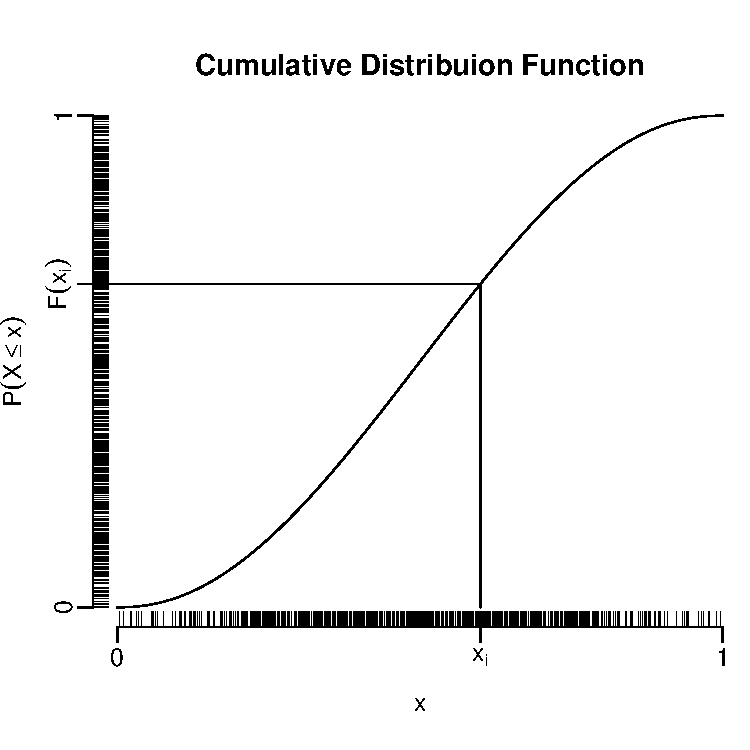
\includegraphics[width=\linewidth]{../cdf_example.pdf}
\captionof{figure}{Finitely supported density data mapped through a beta CDF that maximizes entropy.}
\end{Figure}
To fit arbitrary distance data supported on sets larger than $[0,1]$ to a beta distribution, we reflect the empirical data about zero to satisfy symmetry and rescale to $[0,1]$. 
The transformed data is fitted to a symmetric beta distribution, and the estimate $f$ is half of the distribution transformed back to the scale of the data.
This is similar to what is done to fit a kernel estimate \cite{thompson2012sampling}.
We will refer to this as a half-beta distribution.  
The fourth plot in \figref{duckfits} gives an example of this method fitted to the Anderson and Pospahala duck nest data.

\begin{figure}
  \begin{center}
    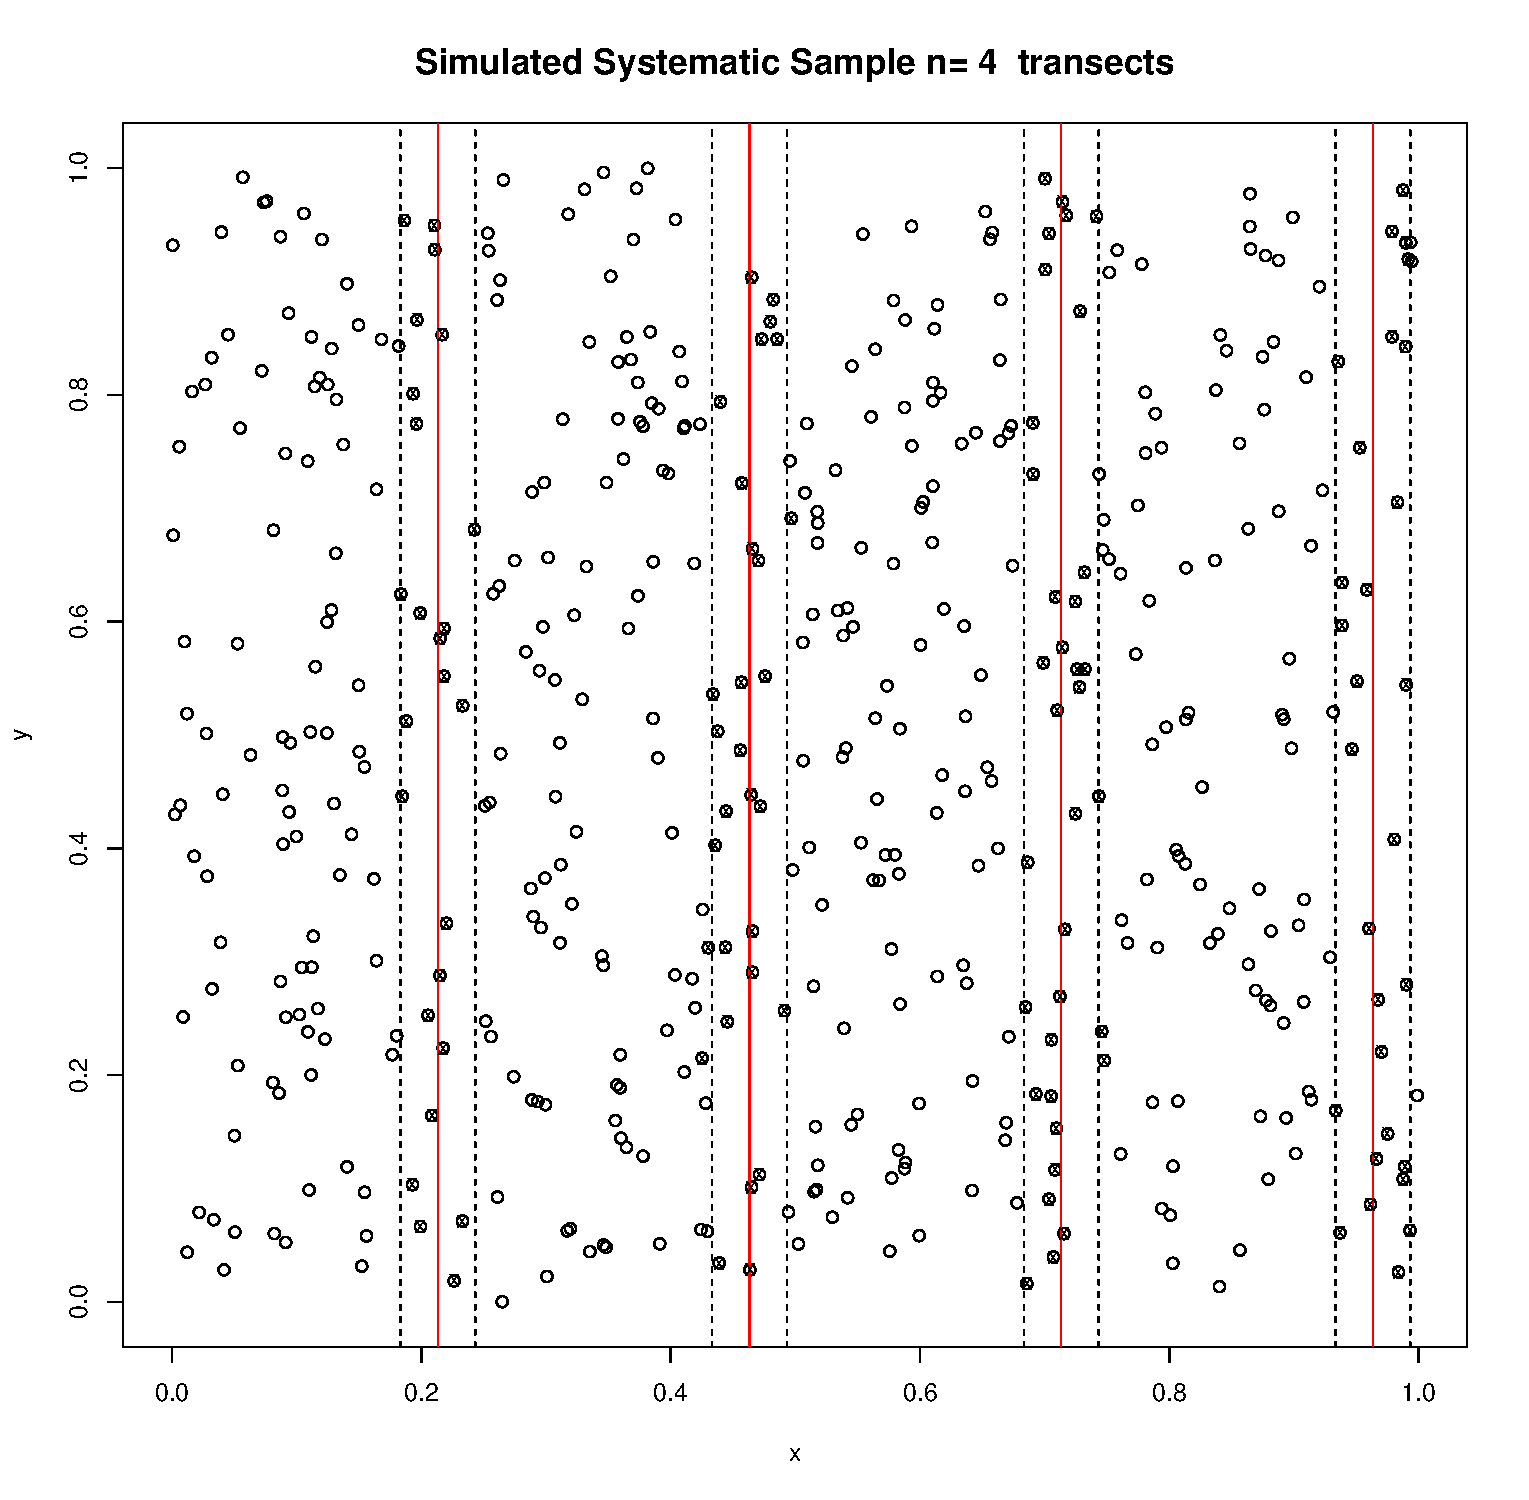
\includegraphics[width=\textwidth]{../simulated_sample.pdf}
    \caption{Simulated systematic sample of size $n=4$ from randomly placed objects in a $1\times 1$ square.}
  \end{center}
\end{figure}
\section{Simulation Comparison}
To quantify a comparison between methods, we simulate systematic transect data on 500 randomly placed points in a $1\times 1$ square.
To mimic Anderson and Pospahala's data, we simulated detection dependent on the perpendicular distance to a transect by Bernoulli trials with probabilities 
  \begin{equation}
    p(d) = 
    \begin{cases}
      1 & |d| < e\\
      (1-d)^p & |d| < b\, e.
    \end{cases}
    \label{detect}
  \end{equation}
In this particular simulation, we choose parameters $p = .65$ and $b = 1.3$ which produces distance samples sufficiently platykurtic. 
See \figref{simulated_densities}.
Since the region has unit area, estimating the density estimates the total $\tau = 500$. 
We conducted 500,000 systematically sampled ($n=4$ equally spaced) ideal bootstraps, and estimated using half-normal estimation, normal kernel estimation with the recommended kernel width \cite{thompson2012sampling}, and EM half-beta estimation with histogram bin sizes given by Sturge's method which is the default histogram break selection in \texttt R. 
An example of a sample is illustrated in \figref{sample}.
The results of the simulation are illustrated in \figref{simulation_results}.
\texttt R codes implementing this simulation can be found at the end of this paper.
\begin{Figure}
  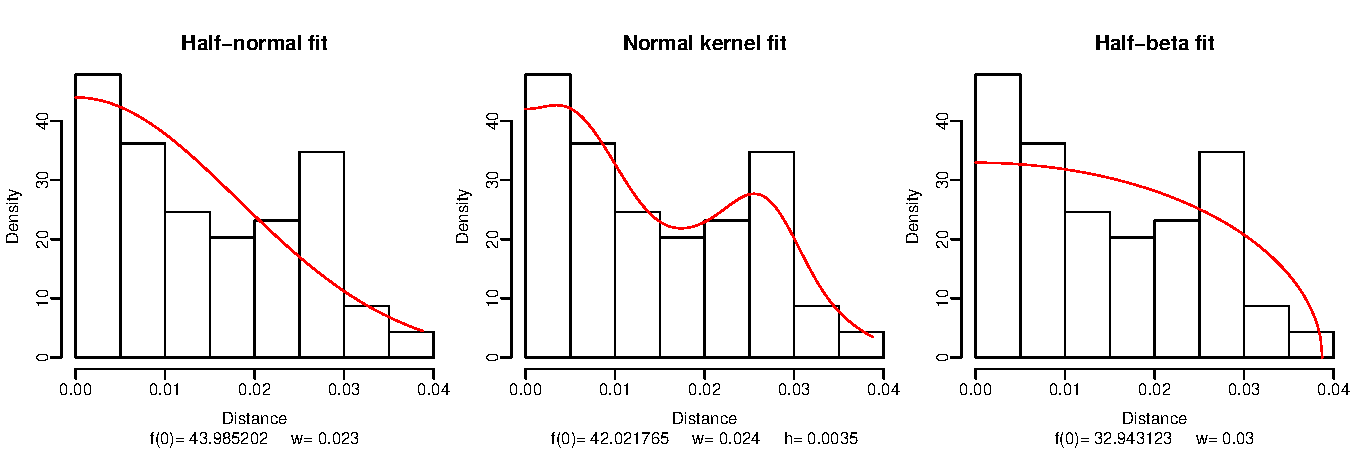
\includegraphics[width=\linewidth]{../problematic_kernel_fit.pdf}
  \captionof{figure}{Simulated detected distance data with various density fits.}
  \label{simulated_densities}
\end{Figure}

\section{Conclusion}
Each estimator has a bimodal distribution to varying degrees.
This source of this is unknown, but it may be due to the piecewise method for defining detectability in \eqref{detect}.  
It may also be inherent to the density estimation, and more work needs to be done to address this question.
The half-normal estimator has a large positive bias. %due to consistently overestimating $\hat f(0)$.
This is likely due to overestimating $\hat f$ near zero, and underestimating in the tails. 
See \figref{duckfits} and \figref{simulated_densities}.
The normal kernel estimate is skewed right, but appears to be relatively unbiased in estimating the total.  
However, it suffers from instability (in terms of mean squared error) likely due to over-fitting as hinted in the introduction.
The EM half-beta estimator has a significantly lower variance than the normal kernel estimator, but appears to have a somewhat significant positive bias.  
Yet, in terms of mean squared error, it still outperforms the non-parametric kernel based estimator.

Note that the EM half-beta curve is constrained to have zero probability at the maximum data value sampled. 
This could be the source the bias in the estimation, and more investigation could reduce this effect and, subsequently, the mean squared error of the estimator.  

In conclusion, the techniques presented in this work give a method for estimating low-kurtosis densities that have potentially lower mean squared errors than two of the most common parametric and non-parametric methods. 
Although biased, further work modeling EM density estimators may result in attractively stable and accurate density estimators.
\end{multicols}

\clearpage
\begin{figure}[h]
  \begin{center}
    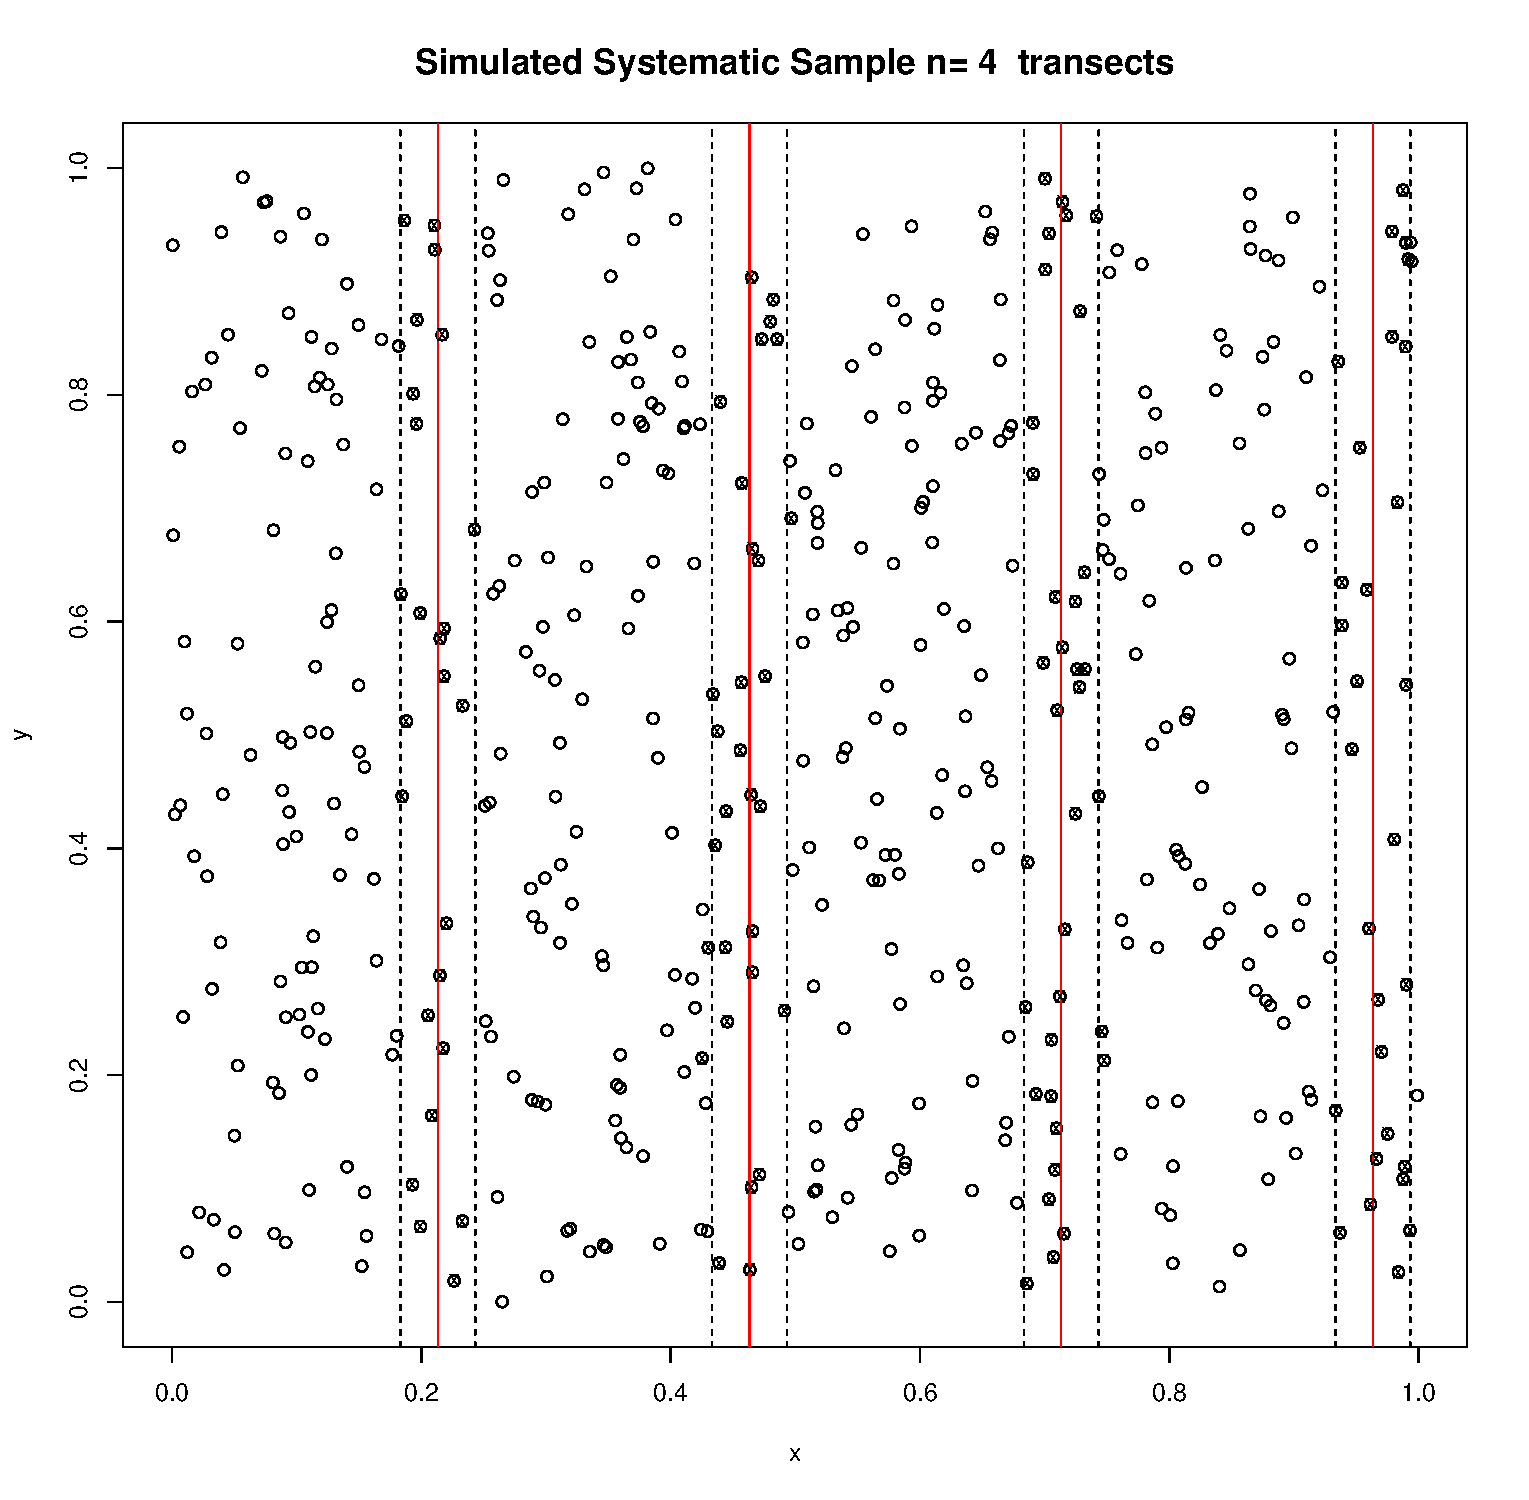
\includegraphics[width=.75\textwidth]{../simulated_sample.pdf}
    \caption{Simulated systematic sample of size $n=4$ from randomly placed objects in a $1\times 1$ square.}
    \label{sample}
  \end{center}
\end{figure}
\begin{figure}[h]
  \begin{center}
  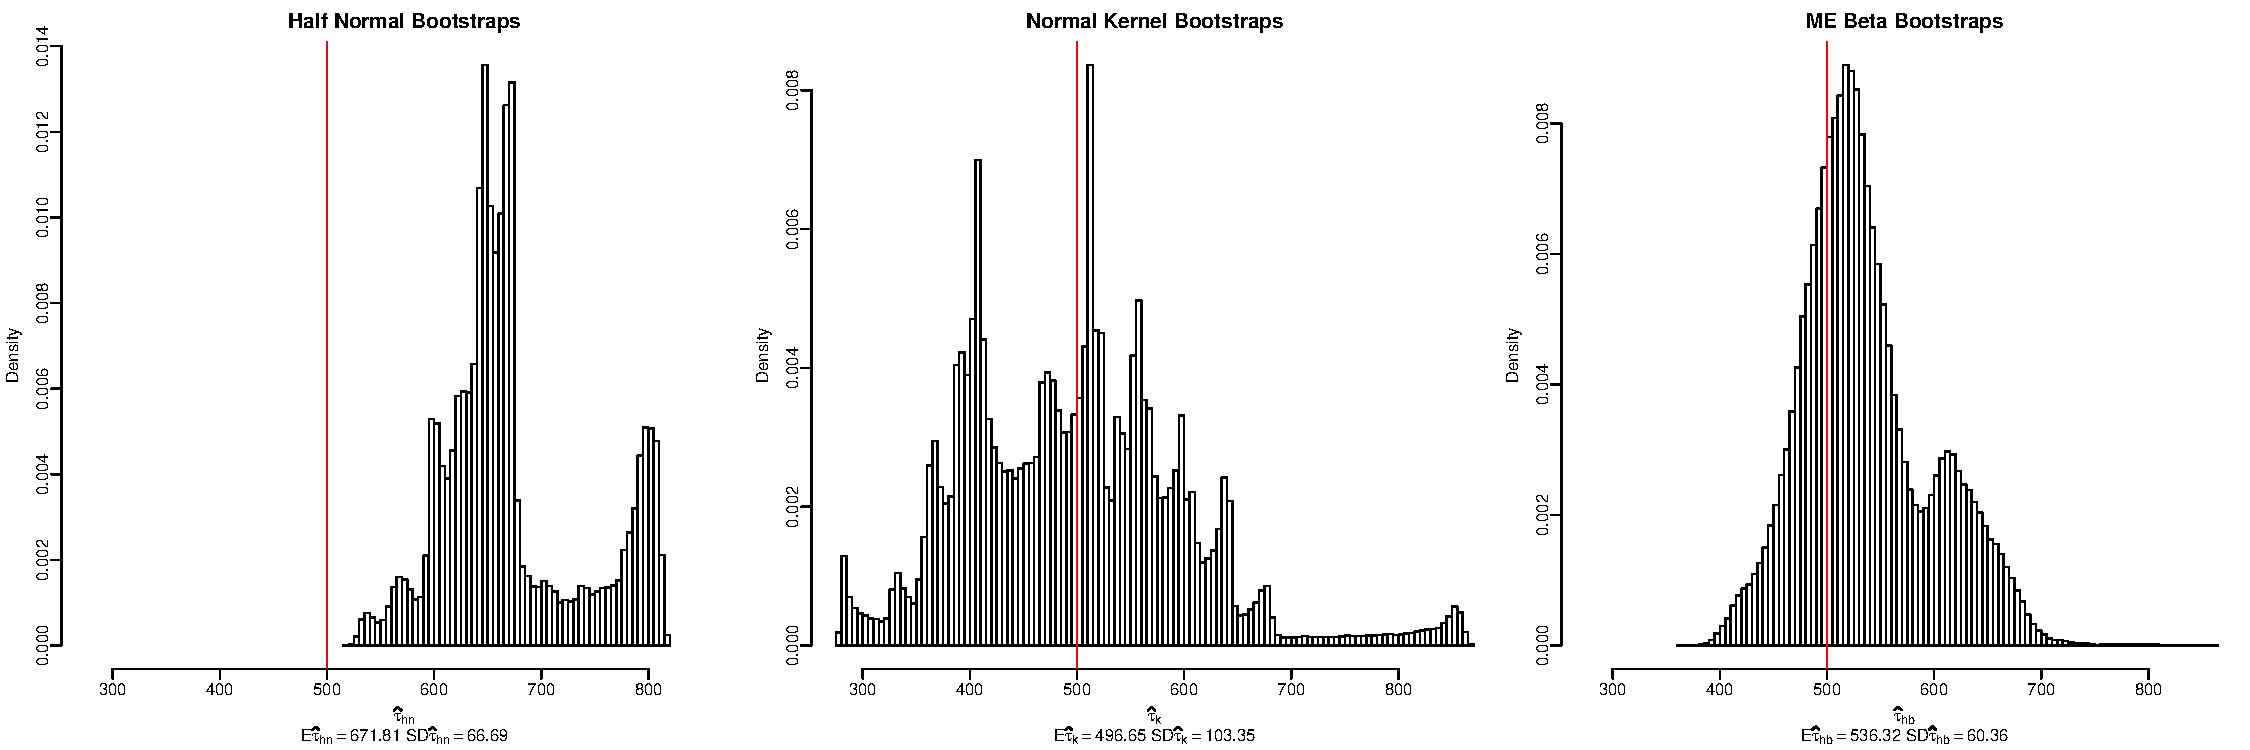
\includegraphics[width=\textwidth]{../500K_bootstrap_comparison.pdf}
  \caption{Density estimation on 500,000 ideal bootstraps on simulated data.}
  \label{simulation_results}
  \end{center}
\end{figure}

\lstset {
	language=R,
	frame=shadowbox,
	basicstyle=\footnotesize\ttfamily, % the size of the fonts that are used for the code
  	backgroundcolor=\color{white},  % choose the background color. You must add \usepackage{color}
  	showspaces=false,               % show spaces adding particular underscores
  	showstringspaces=false,         % underline spaces within strings
  	showtabs=false,                 % show tabs within strings adding particular underscores
  	rulecolor=\color{black},        % if not set, the frame-color may be changed on line-breaks within not-black text (e.g. commens (green here))
  	tabsize=2,                      % sets default tabsize to 2 spaces
  	captionpos=b,                   % sets the caption-position to bottom
  	breaklines=true,                % sets automatic line breaking
  	breakatwhitespace=false,        % sets if automatic breaks should only happen at whitespace
  	keywordstyle=\color{RoyalBlue},      % keyword style
  	commentstyle=\color{YellowGreen},   % comment style
  	stringstyle=\color{ForestGreen}      % string literal style
}

\clearpage
\lstinputlisting[caption=\texttt{estimator\_functions.r}]{../estimator_functions.r}

\lstinputlisting[caption=\texttt{duck\_fits.r}]{../duck_fits.r}

\lstinputlisting[caption=\texttt{simulate\_sample.r}]{../simulate_sample.r}

\nocite{*}
\bibliographystyle{unsrt}
\bibliography{max_entropy_density_estimation} % Use sample.bib as the bibliography file

\end{document}
